\documentclass[11pt,a4paper]{article}
\usepackage[margin=2.7cm]{geometry}
\usepackage{amsmath,amssymb,bm,graphicx,booktabs}
\usepackage[colorlinks=true,linkcolor=blue,citecolor=blue]{hyperref}
\usepackage{enumitem}

\newcommand{\Pir}[1]{\Pi^{(\mathrm r)}_{#1}}
\newcommand{\kt}{k_t}

\title{\vspace{-1.2em}Null tests of the LOS closure-bound estimator:\\
real turbulence, ODT, and a diagnosed initial-condition artifact}
\author{Sparsh Sharma (DLR Braunschweig)\\[0.2em]
\normalsize Working note --- companion to ``What does a line of sight
determine?'' --- \today}
\date{}

\begin{document}
\maketitle
\vspace{-2em}

\paragraph{Summary.} The LOS estimator (previous note: forward map,
realizability cone, per-$\kappa_2$ linear programs) has now been exercised on
two kinds of real line data: (i) an ensemble of lines through DNS of forced
isotropic turbulence (JHTDB), and (ii) ensembles of nominal-HIT ODT
realizations run on DLR CARO with the strain machinery active and
$A_{ij}=0$ --- your false-positive test. Outcome in one sentence:
\emph{the estimator produces no spurious strain signal on either data
source; it did, however, catch a real $\sim$1.5\% component-anisotropy bias
in the ODT initial condition, which we attributed by a reversal experiment
and eliminated by a code fix} --- the eddy mechanism itself passes the null
test cleanly.

\section{Pipeline}

Identical for both data sources. From an ensemble of velocity lines
$\{u_i(y)\}$: cross line-spectra $\phi_{mn}(\kappa_2)$ (all six components)
with jackknife errors; the on-line A1 diagnostics
(T1: $\phi_{11}=\phi_{33}$; T2: vanishing cross spectra); the classical
isotropic longitudinal--transverse derivative relation (T3); and the LP
bounds $[\Pi^-,\Pi^+]$ at three constraint levels (raw; polarization cap
$\gamma=0$; $\gamma=0$ plus log-Lipschitz slope cap $\lambda=4$), with the
measured standard errors entering as inequality bands (T4). Component
energies give $b_{ij}$ (T5). ODT lines use the interior 80\% segment with a
power-normalized Hann window (WALL boundaries); JHTDB lines are periodic.

\section{Real-turbulence null: JHTDB isotropic}

128 lines (1024 points each) through one snapshot of
\texttt{isotropic1024coarse}. Results: T1 splitting exceeds $2\sigma$ in
7\% of wavenumber bins (5\% expected by chance); T2 coherences
$\sim$0.01; T3 holds to $\approx$4\% (quadrature-limited); T4: the bounds
bracket the Crow value $\Pir{ij}=\tfrac45 \kt S_{ij}$ at every constraint
level with widths consistent with the synthetic isotropic calibration.
The component energies give the \textbf{statistical noise floor}: with 128
lines from one snapshot, $b_{ij}$ scatters at $\pm 0.06$ (dominated by the
few independent large-scale structures per snapshot). Strain-generated
anisotropy in the regime of interest is $b\sim0.2$--$0.4$, so the floor is
comfortable, and it shrinks as $1/\sqrt{N}$ with snapshots.

\section{ODT null: nominal HIT on CARO, and what it caught}

Case: the manuscript's homogeneous-strain configuration with
$A_{ij}=0$, dilatation off, eddies on ($\nu=10^{-4}$, $C=7$, $Z=450$,
band-limited isotropic IC, $k_t(0)=1$); 1024 independent realizations per
variant ($\approx$5 minutes wall time each ensemble on one CARO node).

\textbf{What passed immediately.} The estimator brackets the Crow value at
all constraint levels and all times; T1/T2 spectral nulls are clean; the
$t=0$ control is isotropic ($b_{33}=+0.004\pm0.003$).

\textbf{What the pipeline caught.} From $t=0.5$ onward the component
energies showed a small but statistically solid bias:
$b_{33}=+0.0148\pm0.0046$ ($3.2\sigma$), $b_{11}<0$, persistent in sign at
every dump time (figure, left panel). Two facts pointed away from the eddy
dynamics and toward the initial condition: the pattern was
\emph{monotone in the order} $(u,v,w)$, and that is exactly the order in
which the IC whitening was applied --- an ordered Cholesky factor of the
empirical $3\times3$ covariance, which leaves $u$ a pure random-phase
field, orthogonalizes $v$ against $u$, and corrects $w$ against both.

\textbf{Attribution by reversal.} Rebuilding the initializer with the
whitening order permuted to $(w,v,u)$ --- nothing else changed --- flips
the pattern: the $b_{33}$ signal collapses to $+0.002\pm0.004$ and the
over-energized slot moves to $u$ (figure, middle panel). The artifact
follows the ordering, not the physics.

\textbf{Fix and confirmation.} The whitening was replaced by the symmetric
inverse square root $C^{-1/2}$ (Jacobi eigen-decomposition of the
$3\times3$ covariance), which treats the components identically by
construction. With the fixed initializer all three components are within
$\approx1\sigma$ of zero at every time (max $|b_{ii}|=0.005$; figure,
right panel), and every spectral null is clean (T1 exceedances: 0\%).

\begin{figure}[h!]
  \centering
  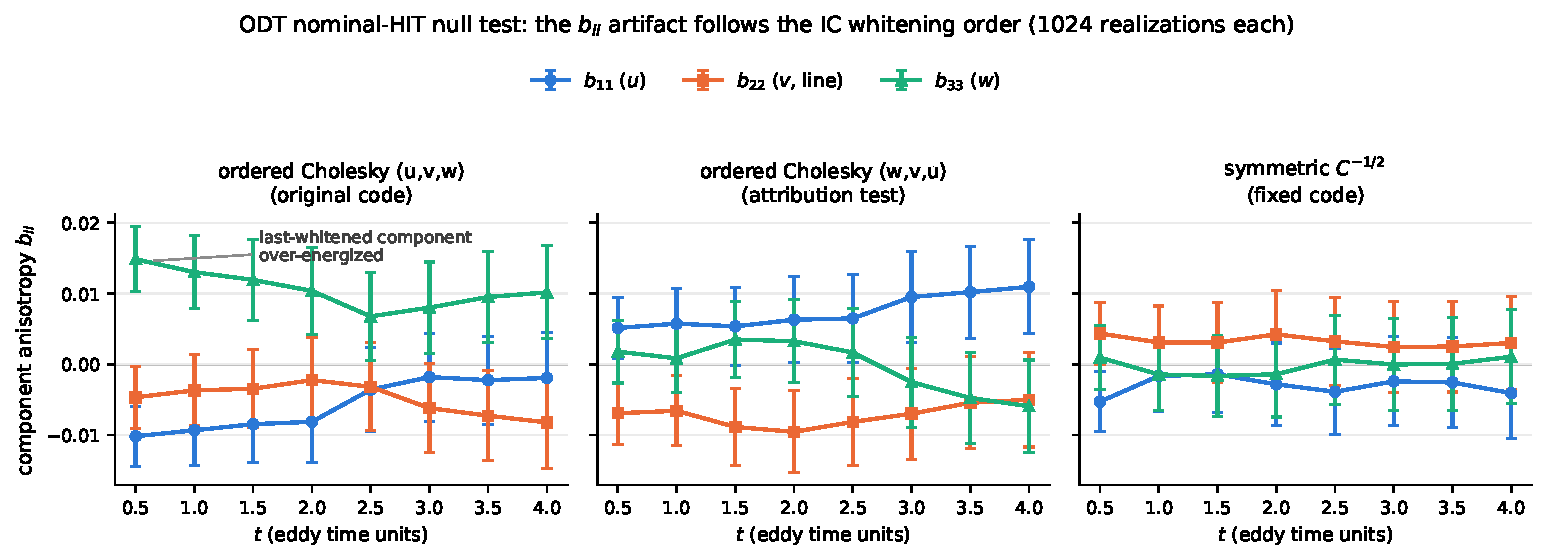
\includegraphics[width=\textwidth]{../post/closure_bound/odt_null/fig_whitening_bt.pdf}
  \caption{Component anisotropy $b_{ii}(t)$ in nominal-HIT ODT, 1024
  realizations per panel, jackknife error bars. Left: original ordered
  Cholesky IC whitening --- the last-whitened component ($w$) is
  over-energized at the 1--1.5\% level and the first ($u$) under-energized.
  Middle: reversing the whitening order flips the pattern, attributing the
  bias to the IC, not the eddy dynamics. Right: symmetric $C^{-1/2}$
  whitening (the code fix) --- all components consistent with isotropy.}
\end{figure}

\section{Implications}

\begin{enumerate}[leftmargin=2em]
\item \textbf{ODT's eddy mechanism generates no false strain signal} in
  nominal HIT at the $\sim$0.5\% level our 1024-realization ensembles
  resolve --- the direct answer to the false-positive question, now with
  the IC artifact removed rather than argued away.
\item \textbf{The estimator pipeline is validated end-to-end on real
  data}, including its error model: the same code that will process
  strained-box DNS lines and strained ODT lines has now run on both data
  types, bracketed the known answers, and demonstrated enough sensitivity
  to find (and localize) a 1\% systematic.
\item \textbf{The artifact episode is itself the strongest sensitivity
  statement}: a component bias twenty times smaller than the strain
  signals of interest was detected, causally attributed by a designed
  intervention, and eliminated. The percent level is exactly where the
  DNS-comparison campaign will operate.
\item \textbf{Bookkeeping for the manuscript}: the published runs used the
  ordered-Cholesky IC. The $\sim$1\% bias is far below the strain-generated
  anisotropy studied there and does not threaten those conclusions, but
  the fixed initializer should be used for all future runs, and the change
  noted.
\end{enumerate}

Next: the strained-box DNS (plane strain, $Sk/\varepsilon\in\{0.8,4,16\}$,
$e\le2$, CARO) supplies the exact $\Pir{ij}$, the true axisymmetric
scalars and their azimuthal residues, and the LOS bound widths under real
distortion --- the quantitative test of the ``weakly constrains''
question that these null tests have now cleared the runway for.

\end{document}
